\documentclass[french,12pt,twoside]{VcCours}

\begin{document}
\Titre{PSI}{Promotion 2021--2022}{Informatique}{TP d'info n°1 -- Algorithmes
de tri et applications.}

\tableofcontents
\separationTitre

\vspace{2cm}
\section*{Objectifs.}
Les algorithmes de tri on pour objectif de modifier le placement des éléments 
d'une liste pour qu'ils soient dans l'ordre (croissant ou décroissant).

\section*{Préliminaires.}

\emph{N'oubliez pas de créer un nouveau répertoire pour ce TP.}

\begin{Exercice}
Créer un fichier \code{TP1.py} dans lequel on écrira toutes les fonctions de ce
TP.

Puis y mettre cette la ligne suivante qui définit une liste \code{L} pour tester
les différents programmes :

\codePython{L = [3,1,0,-2,3,9,2,-6,7,3]}
\end{Exercice}


\newpage
\section{Le tri à bulles.}
\subsection{Algorithme simplifié.}
L'algorithme du tri à bulle consiste à répéter plusieurs fois le traitement 
suivant :

On prends les éléments numéro 0 et 1, on les compare et, s'il ne sont pas dans 
le bon ordre, on les échanges. On fait de même avec les éléments 1 et 2, 
puis 2 et 3,\ldots jusqu'au bout de la liste.

Comme ce traitement fait que le dernier élément de la liste réordonnée se 
retrouve à la bonne place, il suffit d'appliquer $n-1$ fois le traitement 
à la liste de $n$ éléments pour qu'elle soit entièrement triée.

\begin{Exercice}
Créer une fonction \code{unePasseDeTriBulle(L)} qui effectue une seule fois le 
traitement décrit plus haut à la liste \code{L}. Cette fonction modifie la liste 
\code{L}, elle ne retourne donc aucun résultat.

On testera avec 
\end{Exercice}
\begin{Python}
unePasseDeTriBulle(L)
L # doit donner [1,0,-2,3,3,2,-6,7,3,9]
\end{Python}

\begin{Exercice}
Combien de comparaisons fait cette fonction \code{unePasseDeTriBulle} pour une 
liste de $n$ éléments?
\end{Exercice}

\begin{Exercice}
Créer une fonction \code{triBulle(L)} exécutant $n-1$ fois la fonction 
\code{unePasseDeTriBulle(L)}, où $n$ est le nombre d'éléments de la liste 
\code{L}. Cette fonction modifie la liste \code{L}, elle ne retourne donc 
aucun résultat.

On testera avec 
\end{Exercice}
\begin{Python}
triBulle(L)
L # doit donner [-6,-2,0,1,2,3,3,3,7,9]
\end{Python}

\begin{Exercice}
Combien de comparaisons fait cette fonction pour une liste de $n$ éléments?
\end{Exercice}

\subsection{Optimisation : l'algorithme classique.}

On peut optimiser ce tri, car après $k$ application de 
\code{unePasseDeTriBulle(L)}, les $k$ derniers éléments sont à leur place. 
Il n'est donc plus utile de les traiter.

\begin{Exercice}
Modifier \code{unePasseDeTriBulle(L)} en \code{unePasseDeTriBulle(L,n)} pour 
qu'il ne traite que les $n$ premiers éléments de la liste ($n$ n'est plus le 
nombre d'éléments de la liste). Puis modifier 
\code{triBulle(L)} pour qu'il n'applique \code{unePasseDeTriBulle(L,\ldots)} 
que pour les éléments qu'il reste à trier.

On testera avec 
\end{Exercice}
\begin{Python}
triBulle(L)
L # doit donner [-6,-2,0,1,2,3,3,3,7,9]
\end{Python}

\begin{Exercice}
Combien de comparaisons fait cette fonction pour une liste de $n$ éléments?
\end{Exercice}



\section{Le tri par insertion.}
L'idée directrice de l'algorithme de tri par insertion est de prendre un à un 
tous les éléments de la liste de départ et de les insérer dans une nouvelle 
liste de sorte que celle-ci soit toujours triée.

Le principal défi de cette méthode est de savoir insérer un élément dans une 
liste déjà trié de sorte qu'elle reste triée.

\subsection{Détermination de la position d'insertion.}
Si $T$ est une liste triée et $x$ un élément à insérer, pour trouver la position 
à laquelle il doit être inséré, il suffit de partir de la position $0$ et de 
passer à la position suivante tant que ce n'est pas la bonne position. 
Évidemment, on s'arrête parfois à la fin de la liste.

\begin{Exercice}
Créer une fonction \code{positionDInsertion(x,T)} qui donne la position à 
laquelle l'élément \code{x} doit être inséré dans la liste $T$ (qui est supposée 
triée dans l'ordre croissant) pour que la liste reste triée.

On testera avec 
\end{Exercice}
\begin{Python}
T =  [-6,-2,0,1,2,3,3,3,7,9]
positionDInsertion(-20,T) # doit donner 0
positionDInsertion(-6,T) # doit donner 0
positionDInsertion(-1,T) # doit donner 2
positionDInsertion(0,T) # doit donner 2 ou 3
positionDInsertion(3,T) # doit donner 5 ou 6 ou 7 ou 8
positionDInsertion(9,T) # doit donner 9 ou 10
positionDInsertion(20,T) # doit donner 10
\end{Python}

\begin{Exercice}
Combien de comparaisons fait cette fonction pour une liste de $n$ éléments, dans 
le pire des cas ?
\end{Exercice}


\subsection{Tri par insertion.}

\begin{Exercice}
Créer une fonction \code{triInsertion(L)} qui créer une liste \code{T} contenant 
uniquement le premier élément de la liste \code{L}, puis qui, pour chacun des 
autres éléments de la liste \code{L} l'insert dans la liste \code{T} en 
utilisant la fonction précédente.

À la fin, la fonction \code{triInsertion(L)} retourne \code{T}.

On rappelle que \code{T[k:k]=[x]} insert \code{x} à la position \code{k} dans la 
liste \code{T}.

On testera avec 
\end{Exercice}

\begin{Python}
triInsertion(L) # doit donner [-6,-2,0,1,2,3,3,3,7,9]
\end{Python}

\begin{Exercice}
Combien de comparaisons fait cette fonction pour une liste de $n$ éléments?
\end{Exercice}

\subsection{Optimisation : la recherche dichotomique.}

Tel qu'il est programmé ci-dessus, cet algorithme de tri n'est pas plus 
performant que le tri à bulle.

Mais on peut l'améliorer énormément en modifiant la façon dont on cherche la 
position d'insertion.

\medskip
Nous allons faire un recherche dichotomique:
On commence par initialiser deux variables $a$ et $b$, $a$ représente la 
position la plus à gauche et $b$ la plus à droite à laquelle l'élément $x$ est 
susceptible d'être inséré. Puis on pose $c=\lfloor\tfrac{a+b}{2}\rfloor$, et on 
compare $x$ à l'élément qui se trouve à la position $c$ et on modifie $a$ ou $b$ 
en conséquence. (La largueur de l'intervalle $[a;b]$ est à peu près divisée par 
$2$.)

On recommence jusqu'à ce qu'on ait $a=b$, qui est alors la position à laquelle 
$x$ doit être inséré.

\begin{Exercice}
Modifier \code{positionDInsertion(x,T)} pour qu'elle utilise la recherche 
dichotomique.

On testera à nouveau cette fonction, puis \code{triInsertion(L)}.
Combien de comparaisons fait cette fonction pour une liste de $n$ éléments?
\end{Exercice}

Ainsi le tri par insertion à maintenant une complexité (en nombre de 
comparaisons) inférieure à $n\lceil\log_2(n)\rceil$, ce qui est ce qui 
se fait de mieux.

\subsection{Optimisation : tri sur place.}

On dit d'un tri qu'il est "sur place" quand il ne fait que modifier l'ordre des 
éléments de la liste sans créer une autre liste en mémoire. Le tri par insertion 
tel qu'il a été écrit précédemment n'est donc pas un tri sur place.

Le but de l'exercice suivant est donc d'en faire un tri sur place. Pour cela, on 
considérera que la liste \code{L} que les $i$ premiers éléments sont déjà dans 
l'ordre.
\begin{itemize}\renewcommand{\labelitemi}{\textbullet}
  \item au départ, on est sûr que $i=1$ est correct.
  \item on prend le premier élément non trié, et on l'insert dans la partie 
  triée de la liste (autrement dit, le début de la liste). Bien sûr, $i$ 
  augmente alors de $1$.
  \item on recommence le point précédent, jusqu'à avoir trié toute la liste.
\end{itemize}


\begin{Exercice}
Créer \code{positionDInsertion2(x,L,i)} pour qu'elle utilise la recherche 
dichotomique pour positionner $x$ dans la liste des $i$ premier éléments de $L$ 
(la partie triée).

Puis créer \code{triInsertion2(L)} qui fait un tri par insertion sur place.
\end{Exercice}


\newpage
\section{Le tri rapide : quicksort}
\subsection{Présentation}
Le tri rapide "quicksort" est le tri le plus utilisé à l'heure actuel et ce pour 
$4$ raisons :
\begin{enumerate}
  \item Il est optimal en moyenne (mais pas au pire) en nombre de comparaison.
  \item Il est sur place : besoin mémoire minimum.
  \item Il est parallélisable facilement : on peut répartir le calcul sur 
  plusieurs processeurs ou machines.
  \item Il optimise l'usage de la mémoire cache des processeurs.
\end{enumerate}

Cet algorithme est récursif, c'est-à-dire qu'il s'appelle lui-même.

Voici un exemple qui utilise la récursivité : Cette fonction \code{epeler(texte)}
affiche les caractères l'un après l'autre.

(\code{texte[1:]} donne la chaîne privée de son premier caractère.)
\begin{Python}
def epeler(texte):
    """Épelle le texte."""
    if len(texte)<=1 :
        print(texte) 
    else :
        print(texte[0])
        epeler(texte[1:]) 
\end{Python}


\begin{Exercice}
Modifier la fonction en ne changeant que l'ordre des lignes pour que la fonction
épelle le texte à l'envers.

Tester avec \codePython{Epeler("Bidule")}.
\end{Exercice}

\begin{Exercice}
  En s'inspirant de la fonction précédente, écrire une fonction 
  \code{inverser(texte)} qui retourne la chaîne de caractères.
  
  Tester avec \codePython{Epeler("Bidule")}, cela doit retourner \code{"eludiB"}.
\end{Exercice}

\begin{Exercice}
  On dispose d'une liste dont les éléments sont soit des listes soit des éléments.
  
  On souhaite afficher tout le contenu dans l'ordre :

  Par exemple, \code{L=[1,[2,[3,4]],[5,6]]} affiche \code{1 2 3 4 5 6}
  (en allant à la ligne après chaque chiffre).
  
  On rappelle que \code{type([])==list} retourne \code{True}.
  
  Écrire une fonction \codePython{afficher(data)} qui fait cela de façon récursive.
\end{Exercice}
  

\newpage
\subsection{Principe}
Le principe du quicksort est de réorganiser la liste en prenant un pivot (une 
valeur de la liste, souvent la première, mais pas forcément) et en formant trois 
zones : au début les éléments inférieurs au pivot, au milieu ceux égaux au pivot 
et à la fin ceux supérieurs au pivot.

Pour réaliser cette réorganisation, on fait évoluer la liste avec la structure 
suivante :

\medskip
  \begin{center}
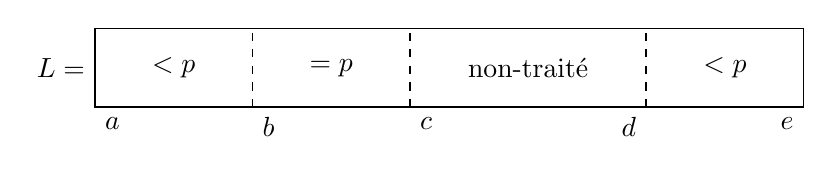
\begin{tikzpicture}[scale=1]
\begin{scope}[semithick]
\draw (0,0) node[anchor=north west]{$a$} --  (2,0)node[anchor=north west]{$b$}  
  --  (4,0)node[anchor=north west]{$c$}  --  (7,0)node[anchor=north east]{$d$}  
  --  (9,0)node[anchor=north east]{$e$} -- (9,1) -- (0,1) -- node[left]{$L=$} cycle;%
\draw[dashed] (2,0) -- (2,1);%
\draw[dashed] (4,0) -- (4,1);%
\draw[dashed] (7,0) -- (7,1);%
\node at (1,.5) {$<p$};%
\node at (3,.5) {$=p$};%
\node at (5.5,.5) {non-traité};%
\node at (8,.5) {$<p$};%
\end{scope}
\end{tikzpicture}
  \end{center}
  
$a$, $b$, $c$ sont les positions du début de chaque zone et  $d$, $e$ les 
positions du dernier élément des zones correspondantes.

L'algorithme est le suivant :
\begin{enumerate}
  \item initialiser $a$, $b$, $c$, $d$ et $e$ judicieusement. Fixer la valeur de 
  $p$.
  \item pour chacun des éléments de la zone triée (jusqu'à ce que $d<c$): on 
  compare l'élément en $c$ au pivot $p$.
  \begin{itemize}
    \item si $<p$ : on échange les éléments $b$ et $c$. On met à jour $b$.
    \item si $>p$ : on échange les éléments $d$ et $c$. On met à jour $d$.
    \item sinon : on met juste $c$ à jour.
  \end{itemize}
\end{enumerate}
 
Pour faire un tri rapide il suffit alors de faire :
\begin{enumerate}
  \item Si la liste a $0$ ou $1$ élément: on ne fait rien.
  \item Sinon :
    \begin{itemize}
    \item On applique l'algorithme précédent.
    \item On relance l'algorithme actuel sur la zone $<p$.
    \item On relance l'algorithme actuel sur la zone $>p$.
  \end{itemize}
\end{enumerate}
 

\subsection{Programmation}
\begin{Exercice}
Écrire une fonction \code{triRapideReorganise(L,debut,fin)} qui réalise le 
premier des deux algorithmes précédents, \code{debut} et \code{fin} repèrent 
la zone de la liste à traiter.

Écrire une fonction \code{triRapideAuxiliaure(L,debut,fin)} qui réalise le 
deuxième des deux algorithmes précédents, \code{debut} et \code{fin} repèrent 
la zone de la liste à traiter.

Puis écrire une fonction \code{triRapide(L)} qui appelle simplement 
\code{triRapideAuxiliaure} avec \code{L}, le premier et le dernier index de la 
liste.

On testera avec 
\end{Exercice}
\begin{Python}
triRapide(L) # doit donner [-6,-2,0,1,2,3,3,3,7,9]
\end{Python}

\subsection{Recherche rapide de la médiane.}
\begin{Exercice}
Écrire une fonction \code{mediane(L)} qui détermine la médiane en utilisant le 
même principe que le quicksort\ldots
\end{Exercice}


\end{document}
